\section{Veruchsaufbau und Durchführung}
\label{sec:Veruchsaufbau}

\begin{figure}[htbp]
    \centering
    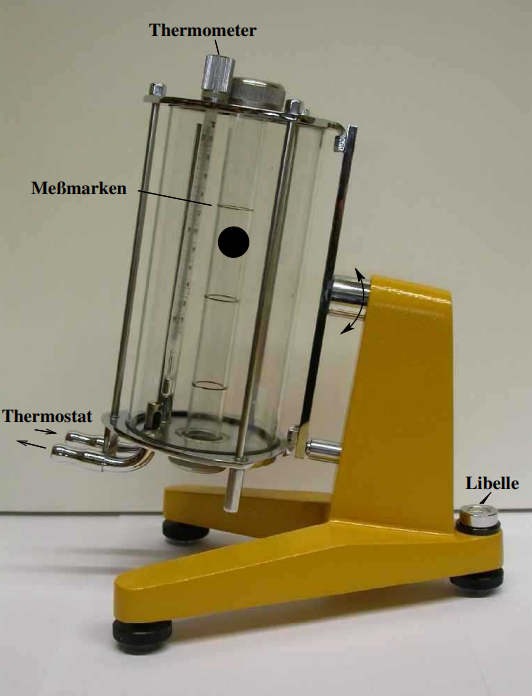
\includegraphics[width=0.7\textwidth]{bilder/hoeppler_viskosimeter.png}
    \caption{Höppler-Viskosimeter\footnote[1]{Bild entnommen aus Versuchsanleitung V107 - Das Kugelfall-Viskosimeter nach Höppler}}
    \label{fig:hoeppler}
\end{figure}

Für die Versuchsdurchführung wird ein Kugelfall-Viskosimeter nach Höppler benötigt. Das Viskosimeter besteht aus einem Zylinder, in den Wasser eingefüllt ist. 
In diesen ist zentral eine Röhre mit drei Messmarkierungen im Abstand von $5\;\unit{cm}$ eingefasst. Das Viskosimeter ist um 180° drehbar.
Das Wasser in dem äußeren Zylinder kann über ein externes Thermostat erhitzt werden. Mit der Libelle und den verstellbaren Füßen lässt sich das Viskosimeter justieren, um
eine eventuelle Schieflage zu korrigieren. In die Röhre wird Wasser eingefüllt. Hierbei ist zu beachten, dass sich keine sichtbaren Luftbläschen bilden.
Damit keine Wirbel entstehen ist es wichtig, dass das Fallrohr leicht schräg ist, damit die Kugel an der Wand herunterrutscht und nicht anschlägt.
\\
Im ersten Teil des Experiments soll die Viskosität von Wasser bei Raumtemperatur bestimmt werden. Hierzu werden 2 verschiedene Kugeln verwendet. Als erstes werden die 
Kugeldurchmesser der kleinen und großen Kugel mit einer Schieblehre bestimmt und notiert. 
\\
Die Fallzeit, die die Kugel für 2 Markierungen, also eine Strecke von $10\;\unit{cm}$, braucht wird für die kleine Kugel mit einer Stoppuhr
gemessen und in einer Tabelle notiert. Ist die Kugel unten angekommen wird das Viskosimeter gedreht.
Da das Viskosimeter bei uns in sich etwas schief war, also die Schräglage bei hoch und runter etwas anders war, haben wir die Zeiten als $t_{runter}$ und $t_{hoch}$ aufgenommen.
Gemessen werden insgesamt 10 Durchgänge.
Zu beachten ist, dass die Kugel zu Beginn der Zeitmessung schon eine konstante Geschwindigkeit hat. Deshalb sollte die Kugel vor Beginn der Zeitmessung schon 2-3cm "gefallen" sein.
\\
Dieser Vorgang wird nun für die große Kugel 5x wiederholt, jedoch mit einer Strecke von $5\;\unit{cm}$.
\\
Im zweiten Teil soll nun die Viskosität von dest. Wasser in Abhängitkeit der Temperatur bestimmt werden. Dazu werden nun stufenweise verschiedene Temperaturen 
von 20°C bis 56°C eingestellt und jeweils 4 Messungen gemacht (2 hoch, 2 runter). Hierbei wird die große Kugel und eine Messstrecke von $5\;\unit{cm}$ verwendet.